\chapter*{\textsc{Introduction}}
\addcontentsline{toc}{chapter}{\textsc{Introduction}}

	\paragraph{} Le but de cette manipulation est d'illustrer la synthèse d'une commande numérique de processus assistée par ordinateur. On utilisera pour cela le logiciel MATLAB/SIMULINK.\\
	On souhaite réaliser l'asservissement en vitesser d'un moteur électrique à commande d'inducteur et courant continu décrit en première approximation par la fonction de transfert entrée-sortie (tension d'alimentation du circuit inducteur/position angulaire de l'arbre moteur).
	\begin{center}
		$ G(p) =\frac{K_G}{p(1+TP)} $
	\end{center}

\paragraph{} où $ K_G \simeq 1 rad . s^{-1} . V^{-1}   $  désigne le gain en vitesse, et $T= 0.1 s $ la constante de temps mécanique.\\
L'objectif est donc d'asservir la vitesse de l'arbre moteur à une valeur de consigne donnée: $e_{ref} = e_1 t$, la variable $ t \in [0,\infty [$ désignant le temps continu. On vise une erreur de traînage nulle en régime permanent, tout en garantissant un comportement dynamique satisfaisant.  

	
	\begin{center}
	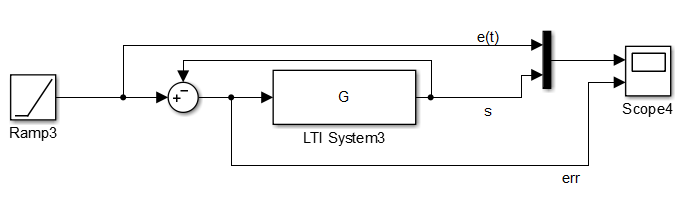
\includegraphics[scale=0.5]{sim1.png}
	\captionof{figure}{\textit{Schema SIMULINK de la boucle fermée \\}}
	\label{fig1} 
	\end{center}   